\def\pathToRoot{./}
%\def\printVersion{}

%%%%%%%%%%%%%%%%
% Document Class
%%%%%%%%%%%%%%%%
\ifcsname printVersion\endcsname%
    \documentclass[compress,handout, dvipsnames]{beamer}
\else%
    \documentclass[compress, dvipsnames]{beamer}
\fi%


%%%%%%%%%%%%%%%
% Packages
%%%%%%%%%%%%%%%
\usepackage{etex}
\usepackage{babel}
\usepackage[utf8]{inputenc}
\usepackage{lmodern}
\usepackage{xifthen}
\usepackage{xstring}
\usepackage{tabu}
\usepackage{graphicx}
\usepackage{booktabs}
\usepackage{relsize}
\usepackage[T1]{fontenc}
\usepackage{mathtools}
\usepackage{csquotes}
\usepackage{stmaryrd}
\usepackage{adjustbox,varwidth} % scaling
\usepackage{wasysym}
\usepackage{censor}
\usepackage{tikz}
\usepackage{tikz-qtree}
\usetikzlibrary{trees, shapes, matrix, calc, positioning, shadows}
\usepackage{soul}
\usepackage{eurosym}
\usepackage[absolute,overlay]{textpos}
\usepackage{transparent}
\usepackage{stackengine}
\usepackage[many]{tcolorbox}
\usepackage{multicol}
\usepackage{pifont}
\usepackage{mathpartir}

%%%%%%%%%%%%%%%
% Configuration
%%%%%%%%%%%%%%%
%Mathe
\newcommand{\mi}[1]{\mathit{#1}}
\newcommand{\with}{\;\middle|\;}
\newcommand{\round}[1]{\left(#1\right)}
\newcommand{\roundd}[1]{(#1)}
\newcommand{\rounddd}[1]{\big(#1\big)}
\newcommand{\roundddd}[1]{\Big(#1\Big)}
\newcommand{\rounddddd}[1]{\bigg(#1\bigg)}
\newcommand{\roundddddd}[1]{\Bigg(#1\Bigg)}
\newcommand{\brackets}[1]{\left[#1\right]}
\newcommand{\curly}[1]{\left\lbrace#1\right\rbrace}
\newcommand{\angles}[1]{\left\langle#1\right\rangle}
\newcommand{\semantics}[2][]{\left\llbracket#2\ifthenelse{\isempty{#1}}{\right\rrbracket}{\right\rrbracket_{#1}}}
\newcommand{\abs}[1]{\left|#1\right|}
\newcommand{\set}[1]{\curly{#1}}
\newcommand{\where}{\,\middle|\,}
\newcommand{\NN}{\mathbb{N}}
\newcommand{\OO}{\mathcal{O}}
\newcommand{\ZZ}{\mathbb{Z}}
\newcommand{\RR}{\mathbb{R}}
\newcommand{\QQ}{\mathbb{Q}}
\newcommand{\ww}{\mathsf{w}}
\newcommand{\ff}{\mathsf{f}}
\newcommand{\lnor}{\mathbin{\overline{\lor}}}
\newcommand{\lnand}{\mathbin{\overline{\land}}}
\newcommand{\universe}{\mathcal{U}}
\newcommand{\powerset}[1]{\mathcal{P}(#1)}

%Beweise
\renewcommand{\qedsymbol}{\ensuremath{\blacksquare}}

% proof rules
\newcommand{\trivialrule}{(\textbf{W})}
\newcommand{\implprule}{(\textbf{$\rightarrow$:Bew})}
\newcommand{\substrule}{(\textbf{Subst})}
\newcommand{\implrule}{(\textbf{Impl})}
\newcommand{\faprule}{(\textbf{$\forall$:Bew})}
\newcommand{\faurule}{(\textbf{$\forall$:Anw})}
\newcommand{\exprule}{(\textbf{$\exists$:Bew})}
\newcommand{\exurule}{(\textbf{$\exists$:Anw})}
\newcommand{\andprule}{(\textbf{$\wedge$:Bew})}
\newcommand{\andurule}{(\textbf{$\wedge$:Anw})}
\newcommand{\orprule}{(\textbf{$\vee$:Bew})}
\newcommand{\implurule}{(\textbf{$\rightarrow$:Anw})}
\newcommand{\cdrule}{(\textbf{FU})}
\newcommand{\hcdrule}{(\textbf{H-FU})}
\newcommand{\transrule}{(\textbf{($\rightarrow$:Bew)}-2)}
\newcommand{\contradictrule}{(\textbf{Widersp.})}
\newcommand{\contraposrule}{(\textbf{KontraP.})}
\newcommand{\eqsubstrule}{(\textbf{$=$-Subst})}
\newcommand{\eqreflrule}{(\textbf{$=$-Refl})}
\newcommand{\triviallabel}{\RightLabel{\footnotesize\trivialrule{}}}
\newcommand{\implplabel}[1][]{\RightLabel{\footnotesize\implprule{}$_{\text{#1}}$}}
\newcommand{\substlabel}[1][]{\RightLabel{\footnotesize\substrule{}$_{\text{#1}}$}}
\newcommand{\impllabel}{\RightLabel{\footnotesize\implrule{}}}
\newcommand{\faplabel}{\RightLabel{\footnotesize\faprule{}}}
\newcommand{\faulabel}{\RightLabel{\footnotesize\faurule{}}}
\newcommand{\explabel}{\RightLabel{\footnotesize\exprule{}}}
\newcommand{\exulabel}{\RightLabel{\footnotesize\exurule{}}}
\newcommand{\andplabel}{\RightLabel{\footnotesize\andprule{}}}
\newcommand{\andulabel}{\RightLabel{\footnotesize\andurule{}}}
\newcommand{\orplabel}{\RightLabel{\footnotesize\orprule{}}}
\newcommand{\implulabel}{\RightLabel{\footnotesize\implurule{}}}
\newcommand{\cdlabel}{\RightLabel{\footnotesize\cdrule{}}}
\newcommand{\hcdlabel}{\RightLabel{\footnotesize\hcdrule{}}}
\newcommand{\translabel}{\RightLabel{\footnotesize\transrule{}}}
\newcommand{\contradictlabel}{\RightLabel{\footnotesize\contradictrule{}}}
\newcommand{\contraposlabel}{\RightLabel{\footnotesize\contraposrule{}}}
\newcommand{\eqsubstlabel}[1][]{\RightLabel{\footnotesize\eqsubstrule{}$_{\text{#1}}$}}
\newcommand{\eqrefllabel}[1][]{\RightLabel{\footnotesize\eqreflrule{}$_{\text{#1}}$}}

\newcommand{\TextRuleName}[1]{\RightLabel{{\footnotesize \textbf{#1}}}}

% Füge zuverlässig eine Leerseite ein:
\newcommand{\blankpage}{\newpage\mbox{}}


% Language
\uselanguage{English}
\languagepath{English}
%\deftranslation[to=German]{Corollary}{Korollar}

% The todo command
\ifcsname showVersion\endcsname%
	\newcommand{\todo}[1]{}
\else \ifcsname printVersion\endcsname%
	\newcommand{\todo}[1]{}
\else%
	\newcommand{\todo}[1]{\begin{alertblock}{TODO}#1\end{alertblock}}
\fi\fi%

% Tikz
\tikzset{
    normal/.style={draw, semithick},
    n/.style={style=normal, circle, inner sep=1mm, minimum size=8mm},
    l/.style={style=normal, rounded corners=1mm, inner sep=1mm, minimum size=6mm},
    e/.style={style=normal, shorten >=1mm, shorten <=1mm, ->},
    syntax/.style={style=normal, ellipse, minimum height=6mm, minimum width=8mm}, % nodes in syntax trees
    inner/.style={style=normal, minimum size=4mm}, % inner leaves or root in normal trees
    leaf/.style={style=normal, circle, minimum size=4mm}, % leaves in normal trees
    te/.style={style=normal}, % edges in a tree
    be/.style={style=e, dashed} % binding edge
}

\newenvironment{tikzsyntaxtree}[1][]{
    \begin{tikzpicture}[baseline=(current bounding box.north), #1]
    \tikzset{grow=down}
    \tikzset{every tree node/.style={syntax}}
    \tikzset{edge from parent/.style={te, edge from parent path={(\tikzparentnode) -- (\tikzchildnode)}}}
}{
    \end{tikzpicture}
}

% Beamer Metadata Defaults
\institute[UCam]
{
    University of Cambridge
}
\author{Simon Schwarz (sfs48@cam.ac.uk) \\ Markus Kuhn (mgk25@cam.ac.uk)}

% Colors
\definecolor{darkcerulean}{rgb}{0.063661, 0.257392, 0.477463}
\definecolor{scooter}{rgb}{0.161162, 0.775760, 0.885416}
\definecolor{fireenginered}{rgb}{0.757398, 0.151664, 0.177088}
\definecolor{pomegranate}{rgb}{0.927557, 0.260794, 0.138377}
\definecolor{mineshaft}{rgb}{0.199974, 0.200015, 0.199971}
\definecolor{tingray}{rgb}{0.501904, 0.501994, 0.501898}
\definecolor{bluegreen}{rgb}{0.089966, 0.635931, 0.735038}
\definecolor{trinidad}{rgb}{0.859854, 0.307332, 0.048339}
\definecolor{buttercup}{rgb}{0.955223, 0.690239, 0.123137}
\definecolor{mediumturquoise}{rgb}{0.335814, 0.846074, 0.749070}

% Presentation Commands
\newcommand<>{\highlight}[2][primary]{%
\alt#3{\ifthenelse{\equal{#1}{primary}}{{\color{bluegreen}{#2}}}{}%
\ifthenelse{\equal{#1}{secondary}}{{\color{trinidad}{#2}}}{}%
\ifthenelse{\equal{#1}{warning}}{{\color{buttercup}{#2}}}{}%
\ifthenelse{\equal{#1}{blue}}{{\color{darkcerulean}{#2}}}{}%
\ifthenelse{\equal{#1}{red}}{{\color{fireenginered}{#2}}}{}%
\ifthenelse{\equal{#1}{green}}{{\color{mediumturquoise}{#2}}}{}%
\ifthenelse{\equal{#1}{black}}{{\color{black}{#2}}}{}}{#2}}

\newcommand{\correct}{\highlight{\ding{51}}}
\newcommand{\incorrect}{\highlight[secondary]{\ding{55}}}
\newcommand{\good}[1]{\textcolor{bluegreen}{#1}}
\newcommand{\medium}[1]{\textcolor{orange}{#1}}
\newcommand{\bad}[1]{\textcolor{trinidad}{#1}}

\newcommand{\DisplayScaledProof}{\maxsizebox{\linewidth}{!}{\DisplayProof}}

\newcommand{\chunk}[1]{\input{\pathToRoot slides/chunks/#1}}
\newcommand{\image}[2][]{\includegraphics[width=#1\textwidth]{\pathToRoot res/#2}}
\newcommand{\fimage}[2][]{\includegraphics[#1]{\pathToRoot res/#2}}
\newcommand{\source}[1]{\vspace{-0.375cm}\hspace*{0pt}\hbox{\fontsize{2}{0} \selectfont\thinspace{\url{#1}}}}
\newcommand{\tsource}[1]{\vspace{-0.375cm}\hspace*{0pt}\hbox{\fontsize{2}{0} \selectfont\thinspace{#1}}}

\makeatletter
\newcommand*{\bufferchunk}[1]{{\beamer@inlecturefalse\input{\pathToRoot slides/chunks/#1}}}
\makeatother

%%%%%%%%%%%%%%%
% Theme
%%%%%%%%%%%%%%%
\usetheme{Boadilla}
\useoutertheme[subsection=false]{miniframes}
\useinnertheme{default}
\usefonttheme{serif}
\usepackage{palatino}
\setbeamerfont{titlelike}{shape=\scshape}
\setbeamerfont{frametitle}{shape=\scshape}
\setbeamercolor*{normal text}{fg=black,bg=white}
\setbeamercolor*{alerted text}{fg=fireenginered}
\setbeamercolor*{example text}{fg=black}
\setbeamercolor*{structure}{fg=black}
\setbeamercolor*{section in head/foot}{fg=white, bg=darkcerulean}
\setbeamercolor*{frametitle}{fg=darkcerulean, bg=white}
\setbeamercolor*{titlelike}{fg=white,bg=darkcerulean}
\setbeamercolor*{palette tertiary}{fg=black,bg=black!10}
\setbeamercolor*{palette quaternary}{fg=black,bg=black!10}

\setbeamertemplate{logo}{
    \vspace{-1em}
    \begin{tikzpicture}
        %\node[anchor=south west, inner sep=0] (X) at (0,0){\includegraphics[height=0.75cm]{\pathToRoot res/logo-cispa.png}};
        \node[] (Z) at (0.36,0.36){{\small\color{black}\insertframenumber}};
    \end{tikzpicture}
}
\newcommand{\nologo}{\setbeamertemplate{logo}{}} % command to set the logo to nothing

\setbeamertemplate{footline}{}
\beamertemplatenavigationsymbolsempty
\setbeamertemplate{title page}{
    \begin{center}
        \vspace{3.6em}
        {\LARGE \color{darkcerulean} \inserttitle}\\\vspace{1.6em}
        {\insertauthor}\\\vspace{1em}
        {\footnotesize \insertinstitute}\\\vspace{1em}
        {\insertdate}
    \end{center}
}

\setbeamertemplate{itemize items}{
    \begin{tikzpicture}
        \fill (0,0) circle (2pt);
        \draw (0,0) circle (3pt);
    \end{tikzpicture}
}

\setbeamertemplate{enumerate items}[default]


% #1 – box name
% #2 – left color
% #3 – right color
% #4 – Title (may contain #1)
\newcommand{\newlargebox}[4]{
    \newtcolorbox{#1}[1][]{
        beamer,
        width=\textwidth+7pt,
        enlarge left by=-3pt,
        titlerule=3mm,
        colframe=white,
        coltitle={#2},
        bottom=2pt,
        top=-4pt,
        left=6pt,
        toptitle=2pt,
        bottomtitle=-2pt,
        fonttitle=\bfseries\large,
        adjusted title={#4},
        outer arc=.5mm,
        arc=.5mm,
        no shadow,
        fuzzy shadow={1mm}{-1mm}{-1.2mm}{.7mm}{black!20},
        interior titled code={
          \path [left color = {#2}, right color = {#3}]
          (title.south west) + (8pt, 0) rectangle ++(\textwidth-1pt, 0.02);
        }
      }
}

% #1 – box name
% #2 – color
% #3 – Title (may contain #1)
\newcommand{\newsmallbox}[3]{
    \newtcolorbox{#1}[1][]{
        beamer,
        width=\textwidth+7pt,
        enlarge left by=-3pt,
        titlerule=0mm,
        colframe=white,
        coltitle={#2},
        bottom=2pt,
        top=-4pt,
        left=6pt,
        toptitle=5pt,
        bottomtitle=-2pt,
        fonttitle=\bfseries\large,
        adjusted title={#3},
        outer arc=.5mm,
        arc=.5mm,
        no shadow,
        fuzzy shadow={1mm}{-1mm}{-1.2mm}{.7mm}{black!20},
        interior titled code={}
    }
}

\newtcolorbox{emptybox}[1][]{
    beamer,
    width=\textwidth,
    % enlarge left by=-3pt,
    titlerule=0mm,
    colframe=white,
    coltitle=black,
    bottom=8pt,
    top=-10pt,
    left=6pt,
    notitle,
    adjusted title={},
    outer arc=.5mm,
    arc=.5mm,
    no shadow,
    fuzzy shadow={1mm}{-1mm}{-1.2mm}{.7mm}{black!20},
    interior titled code={}
}


\newlargebox{defaultbox}{darkcerulean}{scooter}{#1}
\newlargebox{alertbox}{fireenginered}{pomegranate}{#1}
\newlargebox{darkbox}{mineshaft}{tingray}{#1}
\newlargebox{graybox}{tingray}{white}{#1}
\newlargebox{examplebox}{mineshaft}{tingray}{Example {\ifthenelse{\equal{#1}{}}{}{(#1)}}}

\newsmallbox{smalldefaultbox}{darkcerulean}{#1}
\newsmallbox{smallgraybox}{gray}{#1}
\newsmallbox{smallalertbox}{fireenginered}{#1}


\setbeamertemplate{theorem begin}{%
    \normalfont\begin{defaultbox}[{%
    \inserttheoremheadfont
    \inserttheoremname% \inserttheoremnumber
    \ifthenelse{\equal{\inserttheoremaddition}{}}{}{~(\inserttheoremaddition)}%
    \inserttheorempunctuation%
}]}
\setbeamertemplate{theorem end}{\end{defaultbox}}

\setbeamertemplate{proof begin}{%
    \normalfont\begin{darkbox}[{%
    \insertproofname
}]}
\setbeamertemplate{proof end}{\end{darkbox}}

%%%%%%%%%%%%%%%
% HACKS
%%%%%%%%%%%%%%%

%****************************************************************************
% The following is a hack to allow the transparent package to be loaded at the
% same time as the tikz package:
% https://tex.stackexchange.com/questions/253401/tikz-and-ctable-incompatibility-gives-error-when-printing/253417#253417
\makeatletter
\begingroup\expandafter\expandafter\expandafter\endgroup
\expandafter\ifx\csname pgfutil@addpdfresource@extgs\endcsname\relax
\else
  \AtBeginDocument{%
    % \pgf@sys@addpdfresource@extgs@plain{%
    \pgfutil@addpdfresource@extgs{%
      \TRP@list
    }%
  }%
  \let\TRP@addresource\relax
\fi
\makeatother

%***************************************************************************************************
% The following magic makes sure that the pnote command produces notes that are displayed in pdfpc:

% create a new file handle
\newwrite\pdfpcnotesfile

% open file on \begin{document}
\AtBeginDocument{%
	\immediate\openout\pdfpcnotesfile\jobname.pdfpc\relax
	\immediate\write\pdfpcnotesfile{[notes]}
}
% define a # http://tex.stackexchange.com/a/37757/10327
\begingroup
	\catcode`\#=12
	\gdef\hashchar{#}%
\endgroup


\def\lastframenumber{0}

% define command \pnote{} that works like note but
% additionally writes notes to file in pdfpc readable format
\newcommand{\pnote}[1]{%
	% keep normal notes working
	\note{#1}%

	% if frame changed - write a new header
	\ifdim\theframenumber pt>\lastframenumber pt
		\let\lastframenumber\theframenumber
		\begingroup
			\let\#\hashchar
			\immediate\write\pdfpcnotesfile{\#\#\# \theframenumber}%
		\endgroup
	\fi

	% write note to file
	\immediate\write\pdfpcnotesfile{\unexpanded{#1}}%
}
% close file on \begin{document}
\AtEndDocument{%
	\immediate\closeout\pdfpcnotesfile
}

%            END OF pdfpc MAGIC
%***************************************************************************************************


%******************************************************************************
% Magic which allows to cross out a frame
% taken from http://tex.stackexchange.com/a/109162
\usetikzlibrary{calc,decorations.pathmorphing,patterns}

\makeatletter

\pgfdeclaredecoration{penciline}{initial}{
    \state{initial}[width=+\pgfdecoratedinputsegmentremainingdistance,auto corner on length=1mm,]{
        \pgfpathcurveto%
        {% From
            \pgfqpoint{\pgfdecoratedinputsegmentremainingdistance}
                            {\pgfdecorationsegmentamplitude}
        }
        {%  Control 1
        \pgfmathrand
        \pgfpointadd{\pgfqpoint{\pgfdecoratedinputsegmentremainingdistance}{10pt}}
                        {\pgfqpoint{-\pgfdecorationsegmentaspect\pgfdecoratedinputsegmentremainingdistance}%
                                        {\pgfmathresult\pgfdecorationsegmentamplitude}
                        }
        }
        {%TO
        \pgfpointadd{\pgfpointdecoratedinputsegmentlast}{\pgfpoint{8pt}{5pt}}
        }
    }
    \state{final}{}
}

%% Environment crossedOutFrame
% behaves like frame, but allows putting a big cross over the slide
% if option animate is given, the slide is crossed out on the last overlay
% TODO: currently it crosses out on the second overlay
\newenvironment{crossedOutFrame}[2][]{
  \def\cofo{#1}
  \begin{frame}{#2}
  }{
    \IfSubStr{\cofo}{animate}{\pause}{ }
    \begin{tikzpicture}[remember picture,overlay,decoration=penciline]
      \draw[decorate,line width=30pt,red!60!black]
      (current page.north west) -- (current page.south east);
      \draw[decorate,line width=30pt,red!60!black]
      (current page.north east) -- (current page.center) -- (current page.south west);
    \end{tikzpicture}
  \end{frame}
}

%******************************************************************************

% should we annotate types in function signatures?
% look julia manual: "performance tips" / styleguide.
% do not overannotate, because youre removing flexibility.
% only needed when controlling dipatch
% for documentation: let annotations stay in documentation, not in the actual source code.
% would it be useful to have "type comments?" --> only for docu, not for dispatch


\usetikzlibrary{arrows,shadows}
\usepackage{pgf-umlsd}
\usepackage{multirow}
\usepackage{pdfpages}
\usepackage{pgffor}
\usepackage{minted}
\usepackage{algorithm} %ctan.org\pkg\algorithms
\usepackage{algpseudocode}
\usepackage[absolute]{textpos}

%\usepackage{pdfpcnotes}

\DeclareMathOperator{\HammingWeight}{HammingWeight}

\title{Modelling cryptographic side-channels \\with Julia types}
\date{June 29, 2021}

\begin{document}

\maketitle

\section*{Side-channels}

\begin{frame}[fragile]{What is a side-channel?}
    \vspace{-1em}
    \begin{columns}
        \begin{column}{0.45\textwidth}
            \begin{center}
                Cryptographic algorithm executed on hardware \\
                \vspace{0.5em}
                
\includegraphics[width=0.55\textwidth]{res/cardopen.png}
            \end{center}
        \end{column}
        \begin{column}{0.1\textwidth}
            \centering
            {\LARGE +}
        \end{column}
        \begin{column}{0.45\textwidth}
            \centering
            Additional information by measuring \highlight{side-channels}:
            \begin{itemize}
                \item Power consumption
                \item Timing information
                \item \ldots
            \end{itemize}
        \end{column}
    \end{columns}

    \begin{center}
        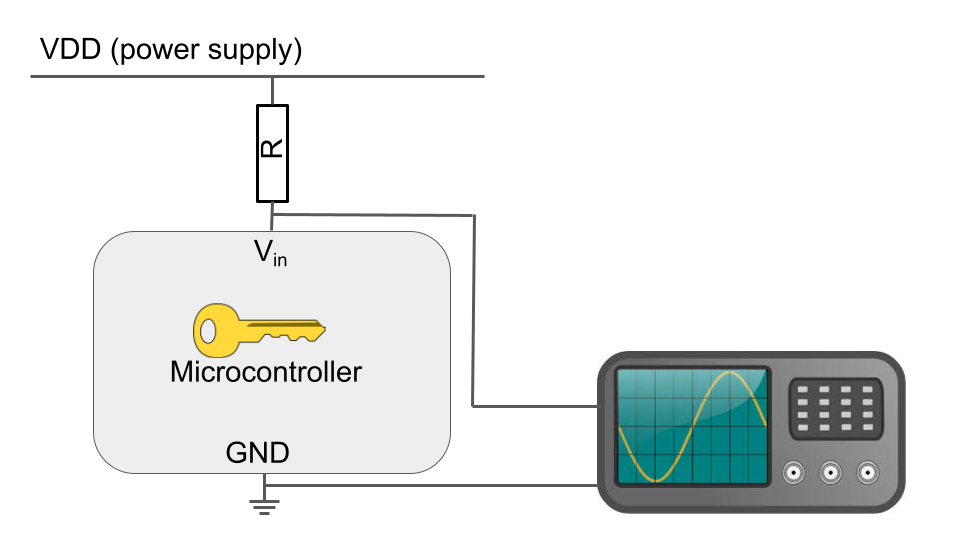
\includegraphics[width=0.7\linewidth]{res/osci1.png}
    \end{center}

\end{frame}

%\begin{frame}[fragile]{Side-channel attacks: Alternative}
%   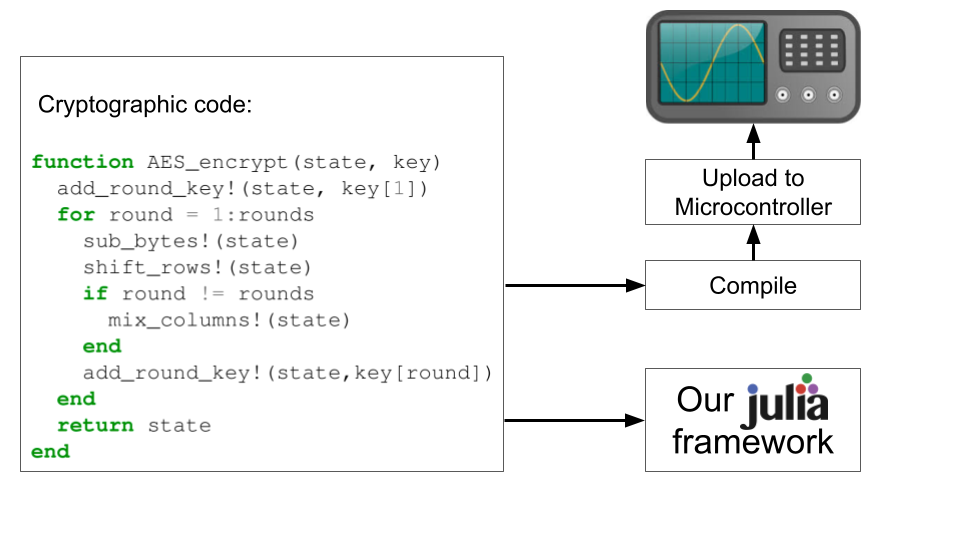
\includegraphics[width=\textwidth]{res/workflow.png}
%\end{frame}

\section*{Our Framework}

\begin{frame}[fragile]{Our framework in Julia}
    Use \highlight{custom types}\only<1>{:} \only<2->{that log all processed values:}
    \vspace{1em}
    \begin{minted}[]{julia}
struct LogInt
    value::Int
end
    \end{minted}
    \pause
\begin{minted}[]{julia}
function Base.:(+)(a::LogInt, b::LogInt)
    result = a.value + b.value
    hamming_weight = count_ones(result)
    println("Recorded $(hamming_weight)")
    return LogInt(result)
end
\end{minted}
\vspace{1em}
\pause
\begin{minted}[]{julia-repl}
julia> a = LogInt(31) + LogInt(2)
Recorded 2
LogInt(33)
\end{minted}
\vspace{-2em}
\hspace{10em}
{\scriptsize $(33)_{10} = (100001)_2$}
\end{frame}

\begin{frame}[fragile]{Collecting side-channel data}

    \begin{minted}[fontsize=\small]{julia-repl}
julia> AES_encrypt([LogInt(42), LogInt(11), ...], [...])
Recorded 2
Recorded 5
Recorded 0
Recorded 5
Recorded 3
Recorded 6
Recorded 7
[~2000 more lines]
        \end{minted}
\vspace{1em}
Should be similar to an oscilloscope recording
\end{frame}


\begin{frame}[fragile]{\texttt{LogInt <: Integer}?}
    Should \texttt{LogInt} be a subtype of \texttt{Integer}? \\

    \textbf{Pros}:
            \begin{itemize}
                \item Code that uses type restrictions to \texttt{Integer} is fine
\begin{minted}[fontsize=\footnotesize]{julia}
AES_encrypt(text::Vector{Integer}, key::Vector{Integer})
\end{minted}
                \item Natural relationship?
            \end{itemize}
    \vspace{0.5em}

    \textbf{Cons}:
            \begin{itemize}
                \item Can introduce ambiguities for multiple dispatch! \\
                    \begin{minted}{julia}
Base.getindex(v::AbstractArray, i::Integer)
                    \end{minted}
                \item Our code can also behave as \texttt{Signed}, \texttt{Unsigned}, \texttt{Int64}, \texttt{Bool} % not exclusively integer
            \end{itemize}

\end{frame}


%\begin{frame}[fragile]{Providing custom methods}
%\begin{columns}
%    \begin{column}{0.45\textwidth}
%        \begin{minted}[fontsize=\tiny]{julia}
%function Base.:(+)(a::LogInt, b::LogInt)
%    result = a.value + b.value
%    hamming_weight = count_ones(result)
%    println("Recorded $(hamming_weight)")
%    return LogInt(result)
%end
%        \end{minted}
%\begin{minted}[fontsize=\tiny]{julia}
%function Base.:(xor)(a::LogInt, b::LogInt)
%    result = xor(a.value, b.value)
%    hamming_weight = count_ones(result)
%    println("Recorded $(hamming_weight)")
%    return LogInt(result)
%end
%    \end{minted}
%    \end{column}
%
%
%    \begin{column}{0.45\textwidth}
%        \begin{minted}[fontsize=\tiny]{julia}
%function Base.getindex(a::Array, b::LogInt)
%    result = a[b.value]
%    hamming_weight = count_ones(result)
%    println("Recorded $(hamming_weight)")
%    return LogInt(result)
%end
%        \end{minted}
%\begin{minted}[fontsize=\tiny]{julia}
%function Base.:(&)(a::LogInt, b::LogInt)
%    result = a.value & b.value
%    hamming_weight = count_ones(result)
%    println("Recorded $(hamming_weight)")
%    return LogInt(result)
%end
%    \end{minted}
%    \end{column}
%\end{columns}
%%\begin{minted}[]{julia}
%%\end{minted}
%\vspace{-1.5em}
%$$\underbrace{\phantom{AAAAAAAAAAAAAAAAAAAAAAAAAAAAAAAAAAAAAAAA}}$$
%\vspace{-2.5em}
%
%\begin{center}
%    Subsume with \highlight{metaprogramming}\visible<2->{:}
%\end{center}
%\pause
%\begin{minted}[fontsize=\small]{julia}
%for op = (:+, :-, :*, :xor, :&, :|)
%eval(
%    function Base.$op(a::LogInt, b::LogInt)
%        result = Base.$op(a.value, b.value)
%        println("Recorded $(count_ones(result))")
%        return LogInt(result)
%    end)
%\end{minted}
%\vspace{-1.5em}
%\hspace{20em}
%{\tiny \textcolor{red}{Warning: simplified syntax}}
%\end{frame}

\begin{frame}[fragile]{Masking}

Store a value $v$ in two shares with
\begin{itemize}
    \item $v = \mathtt{v.val} \oplus \mathtt{v.mask}$ \hspace{1em} ({Boolean masking})
    \item $v = \mathtt{v.val} + \mathtt{v.mask}$ \hspace{1em} ({Arithmetic masking})
\end{itemize}

\vspace{1em}

\begin{minted}[fontsize=\footnotesize]{julia}
@enum MaskType Boolean=1 Arithmetic=2

struct Masked{M, T1, T2}
    val::T1
    mask::T2
end

function Base.(xor)(a::Masked{Boolean}, b::Masked{Boolean})
    Masked{Boolean}(xor(a.val, b.val), xor(a.mask, b.mask))
end

function Base.(+)(a::Masked{Boolean}, b::Masked{Boolean})
    Masked{Boolean}(a.val + b.val, a.mask + b.mask)
end

\end{minted}
\end{frame}

\begin{frame}[fragile]{Masking: Conversion}

\begin{minted}[fontsize=\footnotesize]{julia}
convert(::Type{Masked{Boolean}}, a::Masked{Arithmetic})
    = goubin_a2b(a)
convert(::Type{Masked{Arithmetic}}, a::Masked{Boolean})
    = goubin_b2a(a)
\end{minted}

\begin{thebibliography}{10}
    \beamertemplatebookbibitems
    \bibitem{MaskingConversionGoubin}
    Louis Goubin
    \newblock {A sound method for switching between Boolean and Arithmetic masking}.
\end{thebibliography}
\end{frame}



\begin{frame}[fragile]{Collecting masked side-channel data}

    \begin{minted}[fontsize=\small]{julia-repl}
julia> AES_encrypt([Masked(LogInt(42)), ...], [...])
Recorded 4
Recorded 1
Recorded 6
Recorded 2
Recorded 3
Recorded 6
Recorded 0
[~30000 more lines]
        \end{minted}
\vspace{1em}
Similar to an oscilloscope recording a \textbf{masked version} of our cipher.
\end{frame}

%\begin{frame}[fragile]{Our framework: Summary}
%    \highlight{Ciphers}
%    \begin{itemize}
%        \item AES
%        \item SPECK
%    \end{itemize}
%
%    \highlight{Custom types}
%    \begin{itemize}
%        \item Logging side-channel values
%        \item Countermeasures: Masking
%    \end{itemize}
%
%    \highlight{Attacks} {\scriptsize (recover secret key from side-channel data)}
%    \begin{itemize}
%        \item Differential Power Analysis {\scriptsize (Kocher 1999)}
%        \item Correlation Power Analysis {\scriptsize (Brier et al. 2004)}
%        \item Template Attacks {\scriptsize (Chari et al. 2002)}
%    \end{itemize}
%
%\end{frame}


\section*{Try it yourself}
\begin{frame}[fragile]{Try it out}

    \todo{some very brief summary? timing dependent}
    \begin{center}
        
\includegraphics[width=0.25\linewidth]{res/qr.png} \\
        \vspace{-1em}
        {\footnotesize\url{https://github.com/parablack/CryptoSideChannel.jl}}
    \end{center}

%    \vfill
%    Any open questions left?

\end{frame}

\end{document}

